\section{Iteración VI}
\subsection{Resumen}
Aquí desarrollamos una forma de gestionar proyectos dentro de la aplicación para así crear escenarios dentro de estos.

\subsection{Desarrollo}
Los escenarios generados por la aplicación están agrupados por proyectos, esto debido a que un diseñador de interiores puede realizar varias obras relacionadas entre sí, normalmente cuando son para el mismo cliente. Antes de crear escenarios, es necesario crear proyectos que los contengan y estos proyectos contienen la siguiente información del cliente:
\begin{itemize}
	\item Nombre
	\item Apellido
	\item Teléfono
	\item Email
\end{itemize}

Tras iniciar sesión se muestran los proyectos que han sido creados por el usuario (ver figura x.xx), con la opción de eliminarlos o modificar sus datos (ver figura x.xx). Asimismo el usuario puede agregar un nuevo proyecto ( ver figura x.xx), el cual aparecerá en el listado de proyectos.

Esta funcionalidad cumple cuatro procesos de negocios, correspondientes a las funciones de creación, lectura, actualización y eliminación de proyectos (ver figuras y.yy, y.yy, y.yy y y.yy)

\begin{figure}[h!]
	\centering
	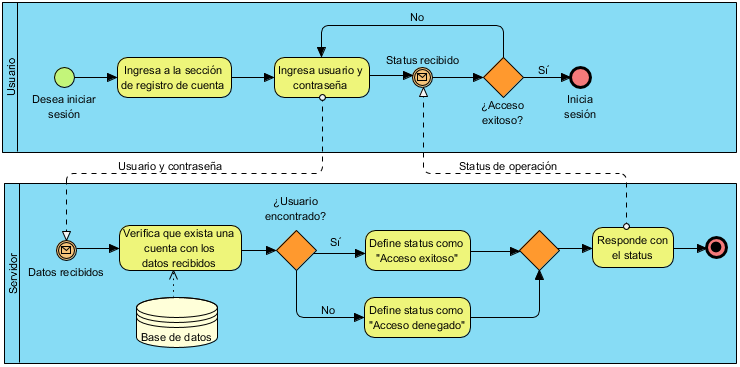
\includegraphics[width=15cm,height=9cm]{imagenes/desarrollo/diagramas/BPMN_LOGIN.png}
	\caption{Diagrama de proceso de recuperación de contraseña.}
	\label{fig:recover}
\end{figure}
\begin{figure}[h!]
	\centering
	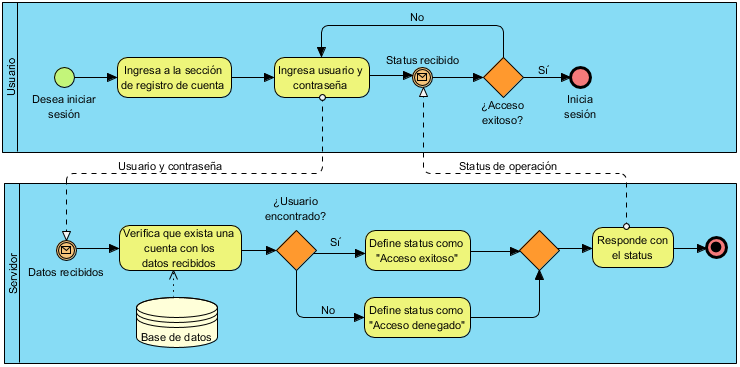
\includegraphics[width=15cm,height=9cm]{imagenes/desarrollo/diagramas/BPMN_LOGIN.png}
	\caption{Diagrama de proceso de recuperación de contraseña.}
	\label{fig:recover}
\end{figure}
\begin{figure}[h!]
	\centering
	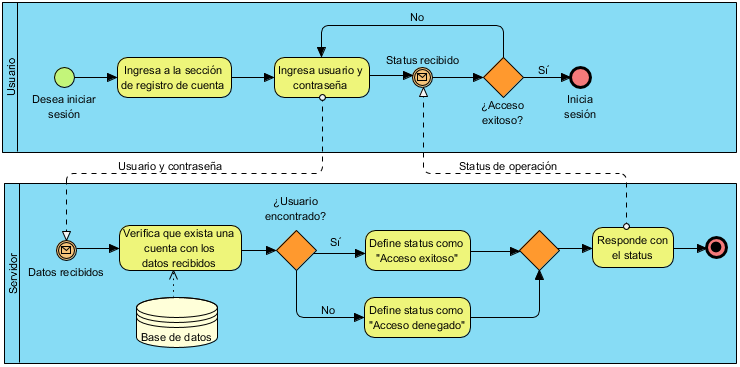
\includegraphics[width=15cm,height=9cm]{imagenes/desarrollo/diagramas/BPMN_LOGIN.png}
	\caption{Diagrama de proceso de recuperación de contraseña.}
	\label{fig:recover}
\end{figure}
\begin{figure}[h!]
	\centering
	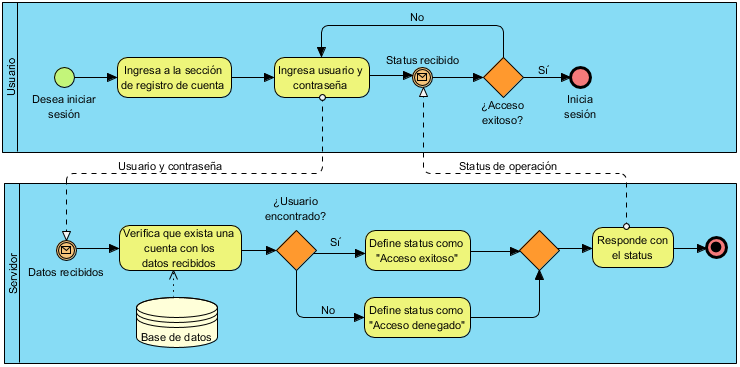
\includegraphics[width=15cm,height=9cm]{imagenes/desarrollo/diagramas/BPMN_LOGIN.png}
	\caption{Diagrama de proceso de recuperación de contraseña.}
	\label{fig:recover}
\end{figure}
\begin{figure}[h!]
	\centering
	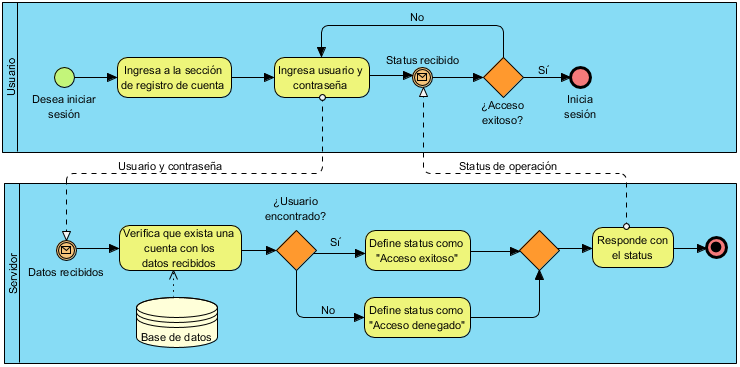
\includegraphics[width=15cm,height=9cm]{imagenes/desarrollo/diagramas/BPMN_LOGIN.png}
	\caption{Diagrama de proceso de recuperación de contraseña.}
	\label{fig:recover}
\end{figure}
\begin{figure}[h!]
	\centering
	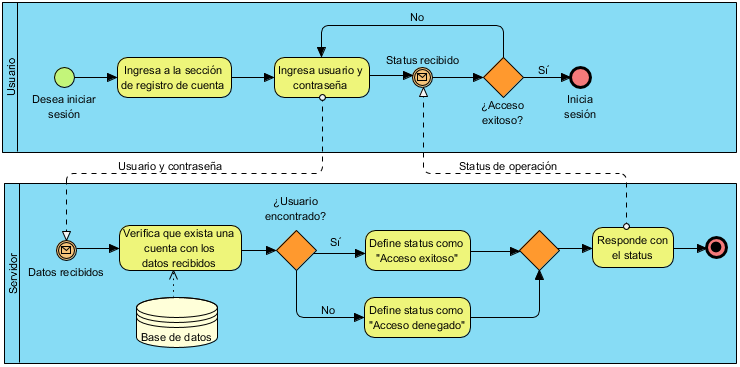
\includegraphics[width=15cm,height=9cm]{imagenes/desarrollo/diagramas/BPMN_LOGIN.png}
	\caption{Diagrama de proceso de recuperación de contraseña.}
	\label{fig:recover}
\end{figure}
\begin{figure}[h!]
	\centering
	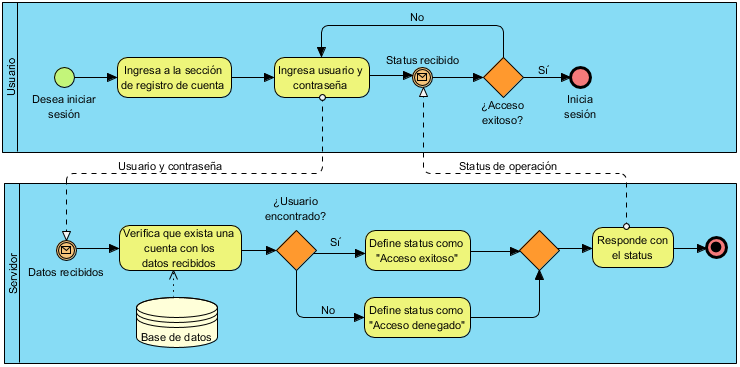
\includegraphics[width=15cm,height=9cm]{imagenes/desarrollo/diagramas/BPMN_LOGIN.png}
	\caption{Diagrama de proceso de recuperación de contraseña.}
	\label{fig:recover}
\end{figure}
